%%% Possible todos:
%%% - Make it clearer what 'robustness' means
%%% - Average distance from the diagonal in the plots (all, and just below):
%%%   1192 6.78926 sentences, average distance below diagonal
%%%   721 12.63 sentences, average distance above diagonal
%%% - deps numbers for all ptb output (do some of the distinctions go away again,
%%%   and so things get closer?)
%%% - Improve the fallback to be smarter (not just an NP bracket always)
%%% - Consider discussing extremely rare constructions, which become a grammar
%%%   rule in a PTB parser, and a crazy category in CCG (but then that category
%%%   isn't used by the parser, as it is below the threshold)

%%% From revierwers:
%%% - Re-pitch the motivation
%%% - Make the details of our method more explicit

%%%  ============================================================================
%%%  
%%%  The paper shows a clear improvement over previous conversion attempts, and
%%%  tackles an important mapping problem between CCG parsing and CFG parsing. The
%%%  evaluation is very interesting.
%%%  
%%%  However, more detail is necessary in explaining what information goes into each
%%%  of the rules for your method (an overview table would be good), and what the
%%%  coverage of the rules is. Just make this a bit more explicit, like you do for
%%%  explaining the C&C parser.
%%%  
%%%  I think it would help the paper to work through the PP/ADVP example in detail
%%%  instead of the discussion of the Italian magistrates example.
%%%  
%%%  Also, please check the following for correctness:
%%%  S[ng]\NP + (S\NP)\(S\NP)
%%%  “coming” + “closer to achieving...” (1)
%%%  “gaining” + “circulation in recent years” (2)
%%%  In Example 1, the correct PTB bracket is a PP,
%%%  while in Example 2 it is an ADVP.
%%%  
%%%  It is not obvious what is the PP in "coming closer to achieving" and the ADVP
%%%  in "gaining circulation in recent years" - do you mean PP in 2 and ADVP in 1?
%%%  
%%%  Also, the number of rules used seems to be in the same order of magnitude as
%%%  number of rules in C&C, although the introduction criticizes C&C for the number
%%%  of hand crafted rules. Please clarify if this is not correct.
%%%  
%%%  At some point, you say "Using sections 00 and 02-21 of the treebanks we
%%%  hand-crafted instructions for 527 lexical categories, including all those used
%%%  by the C&C parser." Are there any additional lexical categories in the treebank
%%%  which the C&C parser doesn't use (but other parsers might use)?
%%%  
%%%  ============================================================================
%%%  
%%%  This paper presents an improvement to previous CCG to PTB transformation
%%%  algorithms. However, one of the motivations of the Clark and Curran paper on
%%%  which this paper was based was to show that the conversion from CCG derivation
%%%  to PTB tree is hard, and that because of this CCG parsers should not be
%%%  evaluated according to PTB trees. We are shown an improved mapping between
%%%  representations but it is not clear that this is a problem that can be solved
%%%  or whether it is needed. The authors should make it clearer whether they
%%%  consider the improvement of this mapping to be an ongoing research goal and why
%%%  it is important when we have other ways of comparing parser output.
%%%  
%%%  The exact contributions are unclear from the paper alone but all rules are
%%%  included in the attached code. The authors are right to warn against reading
%%%  too much into the evaluation in Table 4 and I am especially sceptical about the
%%%  usefulness of the PROJ score. However, while I am not convinced that there is
%%%  any need to judge CCG derivations on the basis of the PTB trees that they can
%%%  generate, I think that this software would be useful to the community as a
%%%  development aid.
%%%  
%%%  ============================================================================
%%%  
%%%  This paper presents a new method for converting CCGBank-style parse tree to
%%%  Penn treebank-style trees. The approach makes use of a large number of
%%%  hand-written transaction procedures, that covert more sentences correctly when
%%%  compared to previous work. Evaluations are performed on gold and automatically
%%%  produced trees and used to compare a number of existing parsers.
%%%  
%%%  This paper presents a well throughout out approach to tree conversion. The use
%%%  of instructions for individual lexical categories (instead of all pairs of
%%%  categories in a parse) is well motivated and interesting. One open question
%%%  that I had was relative to the complexity of writing the instructions/rules. It
%%%  would be helpful to quantify, even anecdotally, how much effort was involved.
%%%  The evaluation is well done and the approach does seem to work better, in terms
%%%  of conversion coverage. However, the CCG parsers still seem to lack behind in
%%%  traditional evaluations and I am left wondering how important that comparison
%%%  is in the first place, given the difference in representations between CCG and
%%%  PTB parsers.
%%%  
%%%  My main complaint with this paper is the informality of Section 3 (Our
%%%  Approach). All of the operations are introduced anecdotally by example.
%%%  Although the examples are very helpful, it would be much better if there were
%%%  some formal specification of the set of possible operations/instructions. The
%%%  inclusion of the source code is helpful, but does not really solve the problem.
%%%  However, this complaint is relatively minor since the overall story was= clear.

\newcommand{\old}{\candc{}-Conv\xspace}

\chapter{Formalism Conversion} \label{chp:conversion}

\begin{center}
\textit{
  A preliminary version of this chapter appeared as \textcite{Kummerfeld-etal:2012:ACL}.
}
\end{center}

In this chapter, we propose an improved, bottom-up method for converting \ccg derivations into \ptb-style phrase structure trees.
In contrast with past work \parencite{Clark-Curran:2009}, which used simple transductions on category pairs, our approach uses richer transductions attached to single categories.
Our conversion preserves more sentences under round-trip conversion (51.1\% \myvs 39.6\%) and is more robust.
In particular, unlike past methods, ours does not require ad-hoc rules over non-local features, and so could be integrated into a parser.

\section{Background}

There has been extensive work on converting parser output for evaluation, \myeg
\textcite{Lin:1998} and \textcite{Briscoe-Carroll-Graham-Copestake:2002} proposed
using underlying dependencies for evaluation.  There has also been work on
conversion to phrase structure, from dependencies \parencite{Xia:2001,Xia:2009} and
from lexicalised formalisms, \myeg \hpsg \parencite{Matsuzaki-Tsujii:2008} and \mytag
\parencite{Chiang:2000,Sarkar:2001}. Our focus is on \ccg to \ptb conversion
\parencite{Clark-Curran:2009}.

\subsection{Combinatory Categorial Grammar (\ccg)}

The lower half of Figure~\ref{fig:ccg-example} shows a \ccg derivation
\parencite{Steedman:2000} in which each word is assigned a {\em category}, and
{\em combinatory rules} are applied to adjacent categories until only one
remains.  Categories can be atomic, \myeg the \cf{N} assigned to
\textit{magistrates}, or complex functions of the form {\em result / arg}, where
{\em result} and {\em arg} are categories and the slash indicates the argument's
directionality.  Combinators define how adjacent categories can combine.
Figure~\ref{fig:ccg-example} uses {\em function application}, where a complex
category consumes an adjacent argument to form its result, \myeg \cf{S[dcl]\bs
NP} combines with the \cf{NP} to its left to form an \cf{S[dcl]}.  More
powerful combinators allow categories to combine with greater flexibility.

\begin{figure}
\small
\begin{tikzpicture}[every text node part/.style={align=center}]

  \node (w0) at (0, 0) {\strut Italian \\ \strut $\cf{N/N}$};
  \node (w1) [right=2ex of w0.east] {\strut magistrates \\ \strut $\cf{N}$};
  \node (w2) [right=2ex of w1.east] {\strut labeled \\ \strut $\cf{((S[dcl]\bs NP)/NP)/NP}$};
  \node (w3) [right=2ex of w2.east] {\strut his \\ \strut $\cf{NP[nb]/N}$};
  \node (w4) [right=2ex of w3.east] {\strut death \\ \strut $\cf{N}$};
  \node (w5) [right=2ex of w4.east] {\strut a \\ \strut $\cf{NP[nb]/N}$};
  \node (w6) [right=2ex of w5.east] {\strut suicide \\ \strut $\cf{N}$};

% PTB above
  \node (nt03) [above=2ex of w3.north] {PRP\$};
  \node (nt04) [above=2ex of w4.north] {NN};
  \node (nt05) [above=2ex of w5.north] {DT};
  \node (nt06) [above=2ex of w6.north] {NN};
  \path (nt03.north) -- node[above=2ex] (nt13-14) {NP} (nt04.north);
  \path (nt05.north) -- node[above=2ex] (nt15-16) {NP} (nt06.north);
  \path (nt13-14.north) -- node[above=2ex] (nt23-26) {S} (nt15-16.north);
  \node (nt20) at (w0 |- nt23-26) {JJ};
  \node (nt21) at (w1 |- nt23-26) {NNS};
  \node (nt22) at (w2 |- nt23-26) {VBD};
  \path (nt20.north) -- node[above=2ex] (nt30-31) {NP} (nt21.north);
  \path (nt22.north) -- node[above=2ex] (nt32-36) {VP} (nt23-26.north);
  \path (nt30-31.north) -- node[above=2ex] (nt40-46) {S} (nt32-36.north);

  \draw (w0.north) -- (nt20.south);
  \draw (w1.north) -- (nt21.south);
  \draw (w2.north) -- (nt22.south);
  \draw (w3.north) -- (nt03.south);
  \draw (w4.north) -- (nt04.south);
  \draw (w5.north) -- (nt05.south);
  \draw (w6.north) -- (nt06.south);
  \draw (nt03.north) -- (nt13-14.south) -- (nt04.north);
  \draw (nt05.north) -- (nt15-16.south) -- (nt06.north);
  \draw (nt13-14.north) -- (nt23-26.south) -- (nt15-16.north);
  \draw (nt20.north) -- (nt30-31.south) -- (nt21.north);
  \draw (nt22.north) -- (nt32-36.south) -- (nt23-26.north);
  \draw (nt30-31.north) -- (nt40-46.south) -- (nt32-36.north);

% CCG below
  \node (c00L) at (w0.south west) {};
  \node (c00R) at (w1.south east) {};
  \draw [-{Straight Barb[length=2mm]}] (c00L) -- node[below=0ex] (c00) {\strut $\cf{N}$} (c00R);
  \node (c01L) at (w3.south west) {};
  \node (c01R) at (w4.south east) {};
  \draw [-{Straight Barb[length=2mm]}] (c01L) -- node[below=0ex] (c01) {\strut $\cf{NP[nb]}$} (c01R);
  \node (c02L) at (w5.south west) {};
  \node (c02R) at (w6.south east) {};
  \draw [-{Straight Barb[length=2mm]}] (c02L) -- node[below=0ex] (c02) {\strut $\cf{NP[nb]}$} (c02R);
  \node (c10L) at (c00L |- c00.south) {};
  \node (c10R) at (c00R |- c00.south) {};
  \draw (c10L) -- node[below=0ex] (c10) {\strut $\cf{NP}$} (c10R);
  \node (c11L) at (w2.west |- c01.south) {};
  \node (c11R) at (w4.east |- c01.south) {};
  \draw [-{Straight Barb[length=2mm]}] (c11L) -- node[below=0ex] (c11) {\strut $\cf{(S[dcl]\bs NP)/NP}$} (c11R);
  \node (c20L) at (w2.west |- c11.south) {};
  \node (c20R) at (w6.east |- c11.south) {};
  \draw [-{Straight Barb[length=2mm]}] (c20L) -- node[below=0ex] (c20) {\strut $\cf{S[dcl]\bs NP}$} (c20R);
  \node (c30L) at (w0.west |- c20.south) {};
  \node (c30R) at (w6.east |- c20.south) {};
  \draw [-{Straight Barb[reversed,length=2mm]}] (c30L) -- node[below=0ex] (c30) {\strut $\cf{S[dcl]}$} (c30R);
\end{tikzpicture}

\caption[A crossing constituents example for \ccg and \ptb.]{ \label{fig:ccg-example}
  A crossing constituents example: \textit{his death a suicide} (\ptb) crosses \textit{labeled his death} (CCGbank).
}
\end{figure}

\begin{table}[t!]
\centering
\begin{tabular}{l|l}
\hline
Categories & Schema \\
\hline\hline
\cf{N} & create an NP \\
\cf{((S[dcl]\bs NP)/NP)/NP} & create a VP \\
\hline
\cf{N/N} + \cf{N} & place left under right \\
\cf{NP[nb]/N} + \cf{N} & place left under right \\
\cf{((S[dcl]\bs NP)/NP)/NP} + \cf{NP} & place right under left \\
\cf{(S[dcl]\bs NP)/NP} + \cf{NP} & place right under left \\
\cf{NP} + \cf{S[dcl]\bs NP} & place both under S\\
\hline
\end{tabular}
\caption[Exmple rules from \textcite{Clark-Curran:2009}.]{ \label{fig:candc09}
  Example \old lexical and rule schemas.
}
\end{table}

We cannot form a \ptb tree by simply relabeling the categories in a \ccg derivation because the mapping to phrase labels is many-to-many, \ccg derivations contain extra brackets due to binarisation, and there are cases where the constituents in the \ptb tree and the \ccg derivation cross (\myeg in Figure~\ref{fig:ccg-example})\footnote{These differences are the result of conscious decisions made in the construction of CCGbank, in many cases enabling the derivation to encode extra dependencies that are not explicitly present in the \ptb}.

\subsection{\textcite{Clark-Curran:2009}}

\textcite{Clark-Curran:2009}, hereafter \old, assign a {\em schema} to each
leaf (lexical category) and rule (pair of combining categories) in the \ccg derivation.
The \ptb tree is constructed from the \ccg bottom-up, creating leaves with
lexical schemas, then merging/adding sub-trees using rule schemas at each step.

The schemas for Figure~\ref{fig:ccg-example} are shown in Table~\ref{fig:candc09}.
These apply to create NPs over \textit{magistrates}, \textit{death}, and
\textit{suicide}, and a VP over \textit{labeled}, and then combine the trees by
placing one under the other at each step, and finally create an S node at the
root.

\old has sparsity problems, requiring schemas for all valid pairs of
categories --- at a minimum, the 2853 unique category combinations found in
CCGbank. \textcite{Clark-Curran:2009} create schemas for only 776 of these,
handling the remainder with approximate catch-all rules.

\old only specifies one simple schema for each rule (pair of
categories).  This appears reasonable at first, but frequently causes
problems, \myeg:

\begin{center}
\cf{(N/N)/(N/N)} + \cf{N/N} \\
\begin{tabular}{ll}
  (1) & ``more than'' + ``30'' \\ % should form a QP
  (2) & ``relatively'' + ``small'' \\ % should from an ADJP
\end{tabular}
%%% ((N/N)/(N/N))\(S[adj]\NP) IN than
%%% (N/N)/(N/N) RB relatively
\end{center}

Here either a QP bracket (1) or an ADJP bracket (2) should be created.  Since
both examples involve the same rule schema, \old would incorrectly process them
in the same way.  To combat the most glaring errors, \old manipulates the \ptb
tree with ad-hoc rules based on non-local features over the \ccg nodes
being combined --- an approach that cannot be easily integrated into a
parser.

These disadvantages are a consequence of failing to exploit the generalisations
that \ccg combinators define.  We return to this example below to show how our
approach handles both cases correctly.

\subsection{\textcite{zhang-zhao-hui:2012:DEMOS}}

\textcite{zhang-zhao-hui:2012:DEMOS} considered a statistical approach to conversion from \ccg to \ptb.
Their system works by classifying each step in the \ccg derivation as either being a \ptb node or being a dummy node, to be flattened in the final structure.
This approach has the limitation that it cannot handle sentences where the structure of the \ccg derivation crosses the structure of the \ptb parse, such as the example in Figure~\ref{fig:ccg-example}.
These cases account for 10\% of sentences, but the method is still fairly effective because they are able to recover most of the structure for such sentences.

\section{Our Approach}

\begin{table}
\centering
\begin{tabular}{lll}
	\hline
		Category & Instruction set \\
	\hline
	\hline
		\cf{N} & (NP$\;$ f) \\[1pt]
		\cf{N/N_1} & (NP$\;$ f$\;$ \{a\}) \\[1pt]
		\cf{NP[nb]/N_1} & (NP$\;$ f$\;$ \{a\}) \\[1pt]
		\cf{((S[dcl]\bs NP_3)/NP_2)/NP_1} & (VP$\;$ f$\;$ a) \\
		 & (VP$\;$ \{f\}$\;$ a) \\
		 & (S$\;$ a$\;$ f) \\
	\hline
\end{tabular}
\caption[Example instructions for our \ccg to \ptb conversion.]{ \label{tab:instructions}
  Instruction sets for the categories in Figure~\ref{fig:ccg-example}.
}
\end{table}

Our conversion assigns a set of instructions to each lexical category and
defines generic operations for each combinator that combine instructions.
Figure~\ref{fig:inst-example} shows a typical instruction, which specifies the
node to create and where to place the \ptb trees associated with the two
categories combining.  More complex operations are shown in
Table~\ref{tab:operators}.  Categories with multiple arguments are assigned one
instruction per argument, \myeg \textit{labeled} has three.  These are applied
one at a time, as each combinatory step occurs.

For the example from the previous section we begin by assigning the
instructions shown in Table~\ref{tab:instructions}.  Some of these can apply
immediately as they do not involve an argument, \myeg \textit{magistrates} has (NP$\;$~f).

One of the more complex cases in the example is \textit{Italian}, which is
assigned (NP~f~\{a\}). This creates a new bracket, inserts the functor's tree, and
flattens and inserts the argument's tree, producing:

\vspace{3mm}
\noindent
(NP (JJ Italian) (NNS magistrates))
\vspace{3mm}

Similar operations apply for the other NPs, followed by a unary rule,
mapping \cf{N} to \cf{NP}.  We handle this by applying one of twelve special
cases for non-combinatory unary operations in CCGbank.

Next \textit{labeled} and \textit{his death} combine.  The verb takes three
arguments, and so has three instructions applied as follows:

\vspace{3mm}
\noindent
(VP (VBD labeled) (NP (PRP\$ his) (NN death))) \\
(VP (VBD labeled) (NP (PRP\$ his) (NN death)) (NP (DT a) (NN suicide))) \\
(S (NP (JJ Italian) (NNS magistrates)) (VP (VBD labeled) (NP (PRP\$ his) (NN death)) (NP (DT a) (NN suicide))))
\vspace{3mm}

As well as creating and flattening, we define three other operators.
The * operator takes the label for the new node from the argument,
\myeg the result of an \cf{S\bs S_1} should correspond to the label of
argument 1 (SINV, SBAR, etc, which all appear as \cf{S} in \ccg).
This is necessary because CCGBank uses additional annotations on categories to distinguish cases that are assigned entirely different labels in the \ptb.
For the complete example above, the final tree is almost correct but omits the S bracket around the two NPs on the right.
To fix our example we could have modified \textit{labeled}'s second instruction to move \textit{his death} under a new S via the final symbol in Table~\ref{tab:operators}.
The subscripts indicate which subtrees to place where.
However, for this particular construction the \ptb annotations are inconsistent, and so we cannot recover without introducing more errors elsewhere.

\begin{figure}
\centering
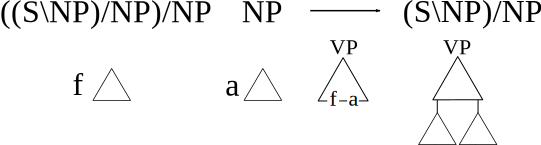
\includegraphics[width=0.85\linewidth]{figures/ccg-example}
\caption[An example function application during \ccg to \ptb conversion.]{ \label{fig:inst-example}
  An example function application.
  Top row: \ccg rule.
  Bottom row: applying instruction (VP f a).
}
\end{figure}

\begin{table}
\centering
\begin{tabular}{lll}
	\hline
		Symbol & Meaning & Example Instruction \\
	\hline
	\hline
		(X f a) & Add an X bracket around functor and argument & (VP$\;$ f$\;$ a) \\
		\{ \} & Flatten enclosed node & (N$\;$ f$\;$ \{a\}) \\
		X* & Use same label as argument or default to X & (S*$\;$ f$\;$ \{a\}) \\
		f$_i$ & Place subtrees &  (PP$\;$ f$_0$$\;$ (S$\;$ f$_{1..k}$$\;$ a)) \\
	\hline
\end{tabular}
\caption[Types of operations in instructions in our \ccg to \ptb conversion.]{\label{tab:operators}
  Types of operations in instructions.
}
\end{table}

For combinators other than function application, we combine the instructions in
various ways.  Additionally, we vary the instructions assigned based on the
\pos tag in 32 cases, and for the word \textit{not}, to recover distinctions
not captured by CCGbank categories alone.  In 52 cases the later
instructions depend on the structure of the argument being picked up.  We have
sixteen special cases for non-combinatory binary rules and twelve special
cases for non-combinatory unary rules.

Our approach naturally handles our QP \myvs ADJP example from the previous section because the two cases
have different lexical categories: {\small\cf{((N/N)/(N/N))\bs (S[adj]\bs NP)}}
on \textit{than} and {\small \cf{(N/N)/(N/N)}} on \textit{relatively}.  This
lexical difference means we can assign different instructions to correctly
recover the QP and ADJP nodes, whereas \old applies the same schema in both
cases because after the first function application for \textit{than}, the category becomes the same as the category for \textit{relaitvely}.

\section{Evaluation}

Using sections 00-21 of the treebanks, we hand-crafted instructions for 527 lexical categories, a process that took under 100 hours, and includes all the categories used by the \candc parser.
There are 647 further categories and 35 non-combinatory binary rules in sections 00-21 that we did not annotate.
For unannotated categories, we use the instructions of the result category with an added instruction.

\begin{table}
\centering
\begin{tabular}{llcccc}
  \hline
    System & Data & P & R & F & Sent. \\
  \hline
  \hline
  % TODO: Move 'len 40' to the left, for a wider table
           & 00 (all)          & 93.67 & 95.37 & 94.51 & 39.6 \\
    \candc & 00 (len $\le 40$) & 94.39 & 95.85 & 95.12 & 42.1 \\
    Conv   & 23 (all)          & 93.95 & 95.33 & 94.64 & 39.7 \\
           & 23 (len $\le 40$) & 94.04 & 95.44 & 94.73 & 41.9 \\
  \hline
           & 00 (all)          & 96.92 & 94.82 & 95.86 & -- \\
    Zhang  & 00 (len $\le 40$) & 97.09 & 95.40 & 96.24 & -- \\
    (2012) & 23 (all)          & 96.67 & 94.77 & 95.71 & -- \\
           & 23 (len $\le 40$) & 96.69 & 94.79 & 95.73 & -- \\
  \hline
           & 00 (all)          & 96.69 & 96.58 & 96.63 & 51.1 \\
    This   & 00 (len $\le 40$) & 96.98 & 96.77 & 96.87 & 53.6 \\
    Work   & 23 (all)          & 96.49 & 96.11 & \textbf{96.30} & \textbf{51.4} \\
           & 23 (len $\le 40$) & 96.57 & 96.21 & 96.39 & 53.8 \\
  \hline
\end{tabular}
\caption{\label{tab:conversion-comparison}
	\parseval Precision, Recall, F-Score, and exact sentence match for converted
	gold \ccg derivations.
}
\end{table}

Table~\ref{tab:conversion-comparison} compares our approach with \old and \textcite{zhang-zhao-hui:2012:DEMOS} on gold \ccg derivations.
The results shown are as reported by \evalb \parencite{Black-etal:1991} using the \textcite{Collins:1997} parameters.
Our approach leads to increases over \old on all metrics of at least 1.1\%, and increases exact sentence match by over 11\% (both absolute).

Many of the remaining errors relate to missing and extra clause nodes and a range of rare structures, such as QPs, NACs, and NXs.
The only other prominent errors are single word spans, \myeg extra or missing ADVPs.
Many of these errors are unrecoverable from CCGbank, either because inconsistencies in the \ptb have been smoothed over or because they are genuine but rare constructions that were lost.

\begin{figure}
\centering
  \hfill
  \scalebox{0.85}{ 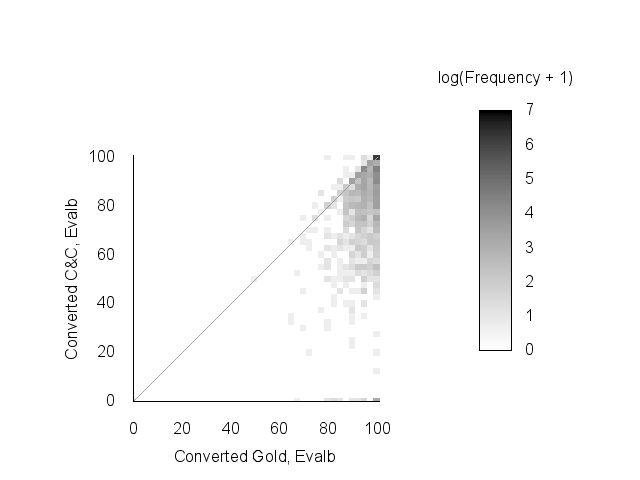
\includegraphics[trim={110mm 25mm 10mm 15mm},clip]{figures/heat-converted} }
  \hfill
  \scalebox{0.85}{ 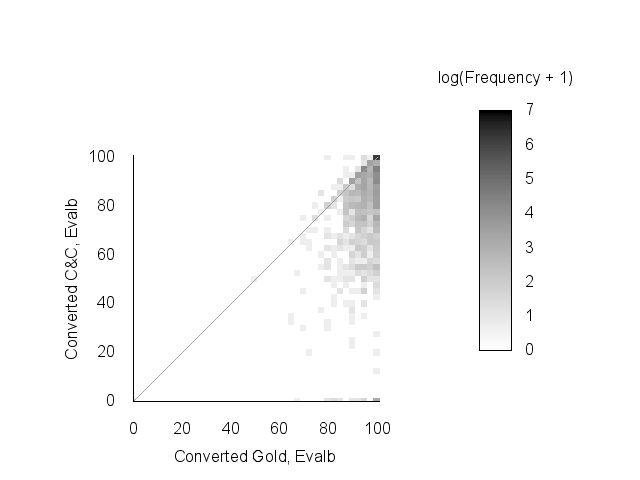
\includegraphics[trim={15mm 0 55mm 40mm},clip]{figures/heat-converted} }
	\\
  \scalebox{0.85}{ 
    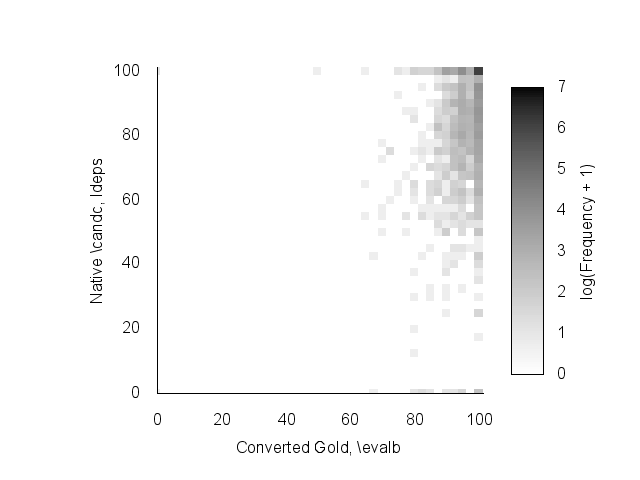
\includegraphics[trim={15mm 0 50mm 40mm},clip]{figures/heat-native}
    \hfill
    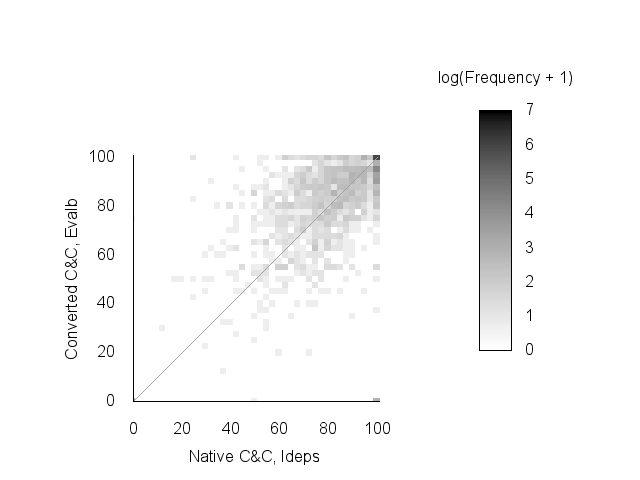
\includegraphics[trim={15mm 0 65mm 40mm},clip]{figures/heat-both}
  }
%%%  \framebox{
%%%  \scalebox{0.6}{ 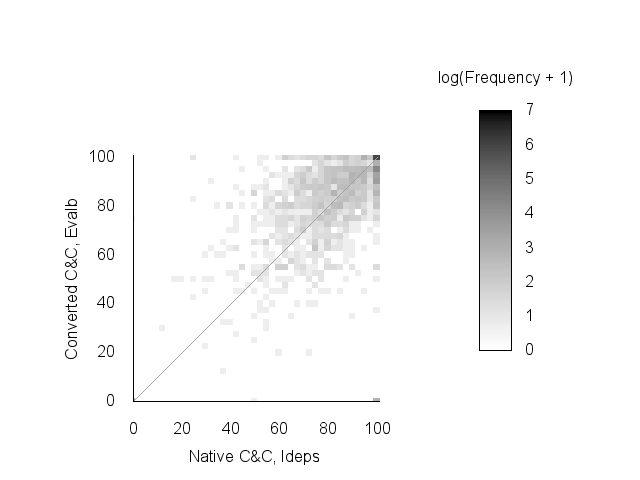
\includegraphics[trim={25mm 0 15mm 0},clip]{figures/heat-both} }
%%%  }
	\caption[Heatmaps comparing gold conversion accuracy, \ccg native evaluation, and converted evaluation.]{ \label{fig:scatter_plots}
		For each sentence in the treebank, we plot the converted parser output against gold conversion (top), the original parser evaluation against gold conversion (left), and the converted parser output against the original parser evaluation against (right).
		A diagonal line indicating $x=y$ is also included.
		Top: Most points lie below the diagonal, indicating that the quality of converted parser output (y) is upper bounded by the quality of conversion on gold parses (x).
		Left: No clear correlation is present, indicating that the set of sentences that are converted best (on the far right), are not necessarily easy to parse.
		Right: In general, accuracy on the native metric is correlated with accuracy after conversion.
	}
\end{figure}

\subsection{Parser Comparison}

When we convert the output of a \ccg parser, the \ptb trees that are produced
will contain errors created by our conversion as well as by the parser. In this
section we are interested in comparing parsers, so we need to factor out errors
created by our conversion.

One way to do this is to calculate a projected score (Proj), as the
parser result over the oracle result, but this is a very rough approximation.
Another way is to evaluate only on the 51\% of sentences for which our
conversion from gold \ccg derivations is perfect (Clean).  However,
even on this set our conversion introduces errors, as when the parser output differs from the gold derivation, it may
contain categories that are harder to convert.

Parser F-scores are generally higher on Clean, which could mean that this
set is easier to parse, or it could mean that these sentences don't contain
annotation inconsistencies, and so the parsers aren't incorrect for returning
the true parse (as opposed to the one in the \ptb).  To test this distinction
we look for correlation between conversion quality and parse difficulty on
another metric.  In particular, Figure~\ref{fig:scatter_plots} (bottom left) shows
\ccg labeled dependency performance for the \candc parser \myvs CCGbank
conversion \parseval scores. The lack of a strong correlation, and the spread
on the line $x=100$, supports the theory that these sentences are not
necessarily easier to parse, but rather have fewer annotation inconsistencies.

In the top plot, the y-axis is \parseval on converted \candc parser output.
Conversion quality essentially bounds the performance of the parser.
The few points above the diagonal are mostly short sentences on which the \candc parser uses categories that lead to one extra correct node (a common case is ADVP v ADJP).
The main constructions on which parse errors occur, \myeg PP attachment, are rarely converted incorrectly, and so we expect the number of errors to be cumulative.
The bottom right plot shows three noteworthy properties, (1) in general the two evaluation metrics are correlated, (2) the \ccg evaluation is slightly harsher, with fewer points below the diagonal line than above it\footnote{This is consistent with prior work, and the fact that \ccg makes some additional distinctions, such as between arguments and adjuncts.}, (3) there are some very common cases on the far right, where the \ccg evaluation is perfect, but conversion mistakes mean the \ptb score is not perfect.
Some sentences are higher in the right plot than the left because there are distinctions in \ccg that are not always present in the \ptb, \myeg the argument-adjunct distinction.

\begin{table}
\centering
\begin{tabular}{lrr|r}
	\hline
	Sentences & Clean & All & Proj \\
	\hline
	\hline
		\multicolumn{2}{l}{Converted gold \ccg} & & \\
		CCGbank & \hspace{0mm}100.0 & \hspace{0mm}96.3 & -- \\
	\hline
		\multicolumn{2}{l}{Converted \ccg} & & \\
		\textcite{Clark-Curran:2007} & 90.9 & 85.5 & 88.8 \\
		\textcite{Fowler-Penn:2010} & 90.9 & 86.0 & 89.3 \\
		\textcite{Auli-Lopez:2011} & 91.7 & 86.2 & 89.5 \\
	\hline
		\multicolumn{2}{l}{Native \ptb} & & \\
		\textcite{Klein-Manning:2003:ACL} & 89.8 & 85.8 & -- \\
		\textcite{Petrov-Klein:2007} & 93.6 & 90.1 & -- \\
		\textcite{Charniak-Johnson:2005} & 94.8 & 91.5 & -- \\
	\hline
\end{tabular}
\caption[F-scores on section 23 for \ptb parsers and \ccg parsers with their output converted by our method.]{ \label{tab:full-comp}
	F-scores on section 23 for \ptb parsers and \ccg parsers with their output converted by our method.
	Clean is only on sentences that are converted perfectly from gold \ccg (51\%).
	All is over all sentences.
	Proj is a projected F-score (All result / CCGbank All result).
}
\end{table}

Table~\ref{tab:full-comp} presents F-scores for three \ptb parsers and three
\ccg parsers (with their output converted by our method).  One interesting
comparison is between the \ptb parser of \textcite{Petrov-Klein:2007} and the
\ccg parser of \textcite{Fowler-Penn:2010}, which use the same underlying
parser.  The performance gap is partly due to structures in the \ptb that are
not recoverable from CCGbank, but probably also indicates that the split-merge
model is less effective in \ccg, which has far more symbols than the \ptb.

It is difficult to make conclusive claims about the performance of the parsers.
As shown earlier, Clean does not completely factor out the errors
introduced by our conversion, as the parser output may be more difficult to
convert, and the calculation of Proj only roughly factors out the
errors.  However, the results do suggest that the performance of the \ccg
parsers is somewhere between the Stanford and Petrov parsers.

\section{Summary}

By exploiting the generalised combinators of the \ccg formalism, we developed a new method of converting \ccg derivations into \ptb-style trees.
Our system is more effective than previous work, increasing exact sentence match by more than 11\% (absolute), and can be directly integrated with a \ccg parser.
The system is available online, see Appendix~\ref{chp:resources}.

%%% Consider pusing the idea that we have found the inconsistencies in the treebank / the sentences that are inconsistent

% Further info on plots

%%%Perfect on gold and deps, but 0 converted
%%%New York City :
%%%New Jersey :
%%%+6 more
%%%Missing an NP bracket over the whole thing (had just an N, which was remoed)
%%%
%%%Moved above the diagonal (from left to right)
%%%100 <100 100
%%%That year the Apple II , Commodore Pet and Tandy TRS-80 came to market .
%%%For the first time , the October survey polled members on imports .
%%%Argentine negotiator Carlos Carballo was in Washington and New York this week to meet with banks .
%%%Mostly just NPs, but is 'to market' an argument of 'came' or a modifier? Parser gets it wrong, but conversion 'fixes' it.
%%% X/PP + PP
%%%     v 
%%%  X   + X\X
%%%prepositions in general

%%%Moved above the diagonal (right plot)
%%%The Japanese industrial companies should know better .
%%%They do n't have plans to cut back .
%%%ADVP v ADJP (is my schema wrong? Or maybe it just gets lucky?)
%%%Ask Matt, is there an inconsistency in the labelling of these sentences?
%%%Is there documentation that makes this difference clearer

%%%Moreover , the Japanese government , now the world's largest aid donor , is
%%%pumping far more assistance into the region than the U.S. is .
%%%Extra nested NPs because of modifier, rather than argument

